\documentclass[t]{beamer}
\usetheme{Copenhagen}
\setbeamertemplate{headline}{} % remove toc from headers
\beamertemplatenavigationsymbolsempty

\usepackage{amsmath, tikz, bm, tkz-euclide,pgfplots}
\pgfplotsset{compat = 1.16}
\usetkzobj{all}

\title{Compound Inequalities}
\author{}
\date{}

\AtBeginSection[]
{
  \begin{frame}
    \frametitle{Objectives}
    \tableofcontents[currentsection]
  \end{frame}
}

\begin{document}

\begin{frame} 
\maketitle
\end{frame}

\section{Solve and graph solutions of compound inequalities}

\begin{frame}{Compound Inequalities -- AND}
	Compound inequalities involve inequalities connected by either the word {\color{blue}\textbf{and}} or the word {\color{red}\textbf{or}}.	\newline\\	\pause
	A number is a solution to a compound inequality that involves the word \emph{and} if it is a solution to \textbf{both} inequalities.
\end{frame}

\begin{frame}{Visual Interpretation of AND}
	\begin{center}
		\[x \geq -1 \textbf{ and } x < 2\]
		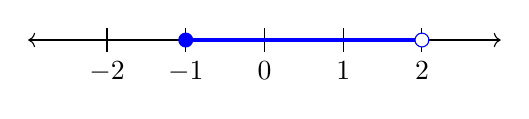
\begin{tikzpicture}
			\draw[<->](-3,0)--(3,0);
			\foreach \x in {-2,-1,...,2}
			\draw(\x,0.15)--(\x,-0.15) node [below] {$\x$};
			\draw[color=blue,fill=blue] (-1,0) circle [radius = 2.5pt];
			\draw[color=blue, ultra thick] (-1,0)--(2,0);
			\draw[color=blue, fill=white] (2,0) circle [radius=2.5pt];
		\end{tikzpicture}	\newline\\
		If you graph each individual inequality, the solution is the part of the number where they overlap.
	\end{center}
\end{frame}

\begin{frame}{Example 1}
	Solve and graph each.	\newline\\
	(a) \quad $-3 < 2x + 1 \leq 3$
	\begin{align*}
		\onslide<2->{-3 &< 2x+1 & 2x+1 &\leq 3} \\[6pt]
		\onslide<3->{-4 &< 2x   & 2x   &\leq 2} \\[6pt]
		\onslide<4->{2x &> -4   & 2x   &\leq 2} \\[6pt]
		\onslide<5->{x  &> -2   &  x   &\leq 1} 
	\end{align*}
	\begin{center}
		\onslide<6->{
			\begin{tikzpicture}
				\draw[<->] (-2.5,0) -- (2.5,0);
				\draw (-1.75,0.15) -- (-1.75,-0.15) node [below] {$-2$};
				\draw (1.75,0.15) -- (1.75,-0.15) node [below] {1};
				\onslide<7->{\draw[->,red,very thick] (-1.75,0.5) -- (2.5,0.5);
						\draw[color=red,fill=white] (-1.75,0.5) circle [radius=2.5pt];}
				\onslide<8->{\draw[->,blue,very thick] (1.75,-0.75) -- (-2.5,-0.75);
						\draw[color=blue,fill=blue] (1.75,-0.75) circle [radius=2.5pt];}
				\onslide<9->{\draw[ultra thick, violet, shorten >=2.5pt, shorten <=2.5pt] (-1.75,0) -- (1.75,0);
						\draw[color=red,fill=white] (-1.75,0) circle [radius=2.5pt];
						\draw[color=blue,fill=blue] (1.75,0) circle [radius=2.5pt];}
						}
			\end{tikzpicture}
	\end{center}
\end{frame}

\begin{frame}{Example 1}
	(b) \quad $1 \leq 2x + 3 < 11$
	\begin{align*}
		\onslide<2->{1 &\leq 2x+3 & 2x+3 &< 11} \\[6pt]
		\onslide<3->{-2 &\leq 2x & 2x &< 8} \\[6pt]
		\onslide<4->{2x &\geq -2 & 2x &< 8} \\[6pt]
		\onslide<5->{x &\geq -1  &  x &< 4} 
	\end{align*}
	\begin{center}
		\onslide<6->{
			\begin{tikzpicture}
				\draw[<->] (-2.5,0) -- (2.5,0);
				\draw (-1.75,0.15) -- (-1.75,-0.15) node [below] {$-1$};
				\draw (1.75,0.15) -- (1.75,-0.15) node [below] {$4$};
				\onslide<7->{\draw[->,red,very thick] (-1.75,0.5) -- (2.5,0.5);
						\draw[color=red,fill=red] (-1.75,0.5) circle [radius=2.5pt];}
				\onslide<8->{\draw[->,blue,very thick] (1.75,-0.75) -- (-2.5,-0.75);
						\draw[color=blue,fill=white] (1.75,-0.75) circle [radius=2.5pt];}
				\onslide<9->{\draw[ultra thick, violet, shorten >=2.5pt, shorten <=2.5pt] (-1.75,0) -- (1.75,0);
						\draw[color=red,fill=red] (-1.75,0) circle [radius = 2.5pt];
						\draw[color=blue,fill=white] (1.75,0) circle [radius=2.5pt];}
						}
			\end{tikzpicture}
	\end{center}
\end{frame}
	
\begin{frame}{Example 1}	
	(c) \quad $2x-7>3$ and $5x-4\leq 6$
	\begin{align*}
		\onslide<2->{2x-7 &> 3 & 5x-4 &\leq 6} \\[6pt]
		\onslide<3->{2x &> 10 & 5x &\leq 10} \\[6pt]
		\onslide<4->{x &> 5 & x &\leq 2} 
	\end{align*}
	\begin{center}
		\onslide<5->{
			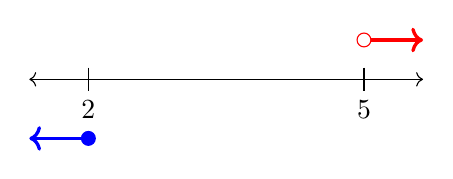
\begin{tikzpicture}
				\draw[<->] (-2.5,0) -- (2.5,0);
				\draw (-1.75,0.15)--(-1.75,-0.15) node [below] {2};
				\draw (1.75,0.15)--(1.75,-0.15) node [below] {5};
				\onslide<6->{\draw[color=red,->,very thick] (1.75,0.5) -- (2.5,0.5);
						\draw[color=red,fill=white] (1.75,0.5) circle [radius=2.5pt];}
				\onslide<7->{\draw[color=blue,->,very thick] (-1.75,-0.75) -- (-2.5,-0.75);
						\draw[color=blue,fill=blue] (-1.75,-0.75) circle [radius=2.5pt];}
						\end{tikzpicture}
						}
	\end{center}

	\onslide<8->{Do not overlap \quad}	\onslide<9->{\textbf{No solution}}
	\end{frame}

\begin{frame}{Compound Inequalities -- OR}
	The word \alert{or} indicates the solution be in {\color{blue}\textbf{either}} inequality (or both).	\newline\\
	\[x > 2 \text{ or } x \leq -1\]
	\begin{center}
		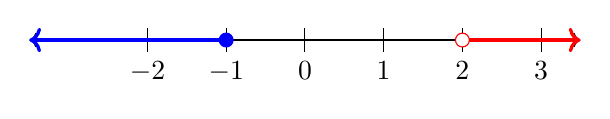
\begin{tikzpicture}
			\draw[<->] (-3.5,0) -- (3.5,0);
			\foreach \x in {-2,-1,...,3}
			\draw (\x,0.15) -- (\x,-0.15) node [below] {$\x$};
			\draw[->,blue,very thick] (-1,0) -- (-3.5,0);
			\draw[color=blue,fill=blue] (-1,0) circle [radius=2.5pt];
			\draw[->,red,very thick] (2,0) -- (3.5,0);
			\draw[color=red,fill=white] (2,0) circle [radius=2.5pt];
		\end{tikzpicture}
	\end{center}
\end{frame}

\begin{frame}{Example 2}
	Solve and graph each.	\newline\\
	(a) \quad $2x-3<7$ or $35-4x \leq 3$
	\begin{align*}
		\onslide<2->{2x-3 &< 7 & 35-4x &\leq 3} \\[6pt]
		\onslide<3->{2x   &<10 &   -4x &\leq -32} \\[6pt]
		\onslide<4->{x    &<5  &     x &\geq 8} 
	\end{align*}
	\begin{center}
		\onslide<5->{
			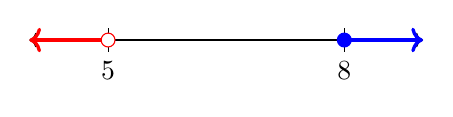
\begin{tikzpicture}
				\draw[<->] (-2.5,0) -- (2.5,0);
				\draw (-1.5,0.15) -- (-1.5,-0.15) node [below] {5};
				\draw (1.5,0.15) -- (1.5,-0.15) node [below] {8};
				\onslide<6->{\draw[->,red,very thick] (-1.5,0)--(-2.5,0);
						\draw[color=red,fill=white] (-1.5,0) circle [radius=2.5pt];}
				\onslide<7->{\draw[->,blue,very thick] (1.5,0) -- (2.5,0);
						\draw[color=blue,fill=blue] (1.5,0) circle [radius=2.5pt];}
			\end{tikzpicture}}
	\end{center}
\end{frame}

\begin{frame}{Example 2}
	(b) \quad $3x-5\leq 13$ or $5x+2>-3$
	\begin{align*}
		\onslide<2->{3x-5 &\leq 13 & 5x+2 &> -3} \\[6pt]
		\onslide<3->{3x &\leq 18 & 5x &> -5} \\[6pt]
		\onslide<4->{x &\leq 6 & x &> -1} 
	\end{align*}
	\begin{center}
		\onslide<5->{
			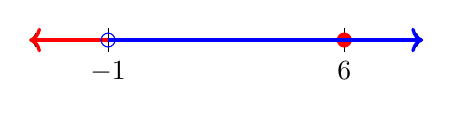
\begin{tikzpicture}
				\draw[<->] (-2.5,0) -- (2.5,0);
				\draw (-1.5,0.15) -- (-1.5,-0.15) node [below] {$-1$};
				\draw (1.5,0.15) -- (1.5,-0.15) node [below] {6};
				\onslide<6->{\draw[->,red,very thick] (1.5,0) -- (-2.5,0);
						\draw[color=red,fill=red] (1.5,0) circle [radius=2.5pt];}
				\onslide<7->{\draw[->,blue,very thick] (-1.5,0) -- (2.5,0);
						\draw[color=blue] (-1.5,0) circle [radius=2.5pt];}
			\end{tikzpicture}}	\newline\\
			\onslide<8->{All Real Numbers}
	\end{center}
\end{frame}

\begin{frame}{Example 2}
	(c) \quad $2x + 5 \leq 3$ or $2x + 3 < 3$
	\begin{align*}
		\onslide<2->{2x+5 &\leq 3 & 2x+3 &< 3} \\[6pt]
		\onslide<3->{2x &\leq -2 & 2x &< 0} \\[6pt]
		\onslide<4->{x &\leq -1 & x &< 0} 
	\end{align*}
	\begin{center}
		\onslide<5->{
			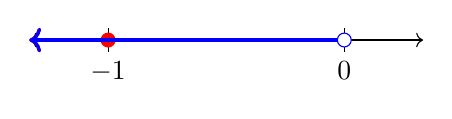
\begin{tikzpicture}
				\draw[<->] (-2.5,0) -- (2.5,0);
				\draw (-1.5,0.15) -- (-1.5,-0.15) node [below] {$-1$};
				\draw (1.5, 0.15) -- (1.5, -0.15) node [below] {0};
				\onslide<6->{\draw[->,red,very thick] (-1.5,0) -- (-2.5,0);
						\draw[color=red,fill=red] (-1.5,0) circle [radius=2.5pt];}
				\onslide<7->{\draw[->,blue,very thick] (1.5,0) -- (-2.5,0);
						\draw[color=blue,fill=white] (1.5,0) circle [radius=2.5pt];}
			\end{tikzpicture}}
			\onslide<8->{\[x < 0\]}
	\end{center}
\end{frame}

\end{document}
